
%%%%%%%%%%%%%%%%%%%%%%%%%%%%%%%%%%%%%%%%%%%%%%%%%%%%%%%%%%%%%
\section{模型的改进与推广}

\subsection{模型的改进}

（1）\textbf{振打同步性约束。}引入同步因子$S=(\sum\delta_i)^2/\sum\delta_i^2$衡量多电场同时振打的风险，$S=4$为完全同步（峰值最大），$S=1$为完全错峰。数据中$T_1/T_2\approx1.003$、$T_3/T_4\approx1.001$，前两电场和后两电场各自同步振打。在优化中增加错峰约束$T_i\neq T_j$或相位错开，降低瞬时排放峰值。

（2）\textbf{贝叶斯参数估计完善。}当前Laplace近似因限幅数据残差非正态，95\% CI覆盖率仅3\%。可改用Bootstrap重采样或MCMC获得更可靠的参数后验分布，在论文中报告参数的置信范围而非仅点估计。

（3）\textbf{振打过频系数$r$标定。}$r=0.5$为工程先验，可结合振打瞬态实验数据或CFD模拟标定$r$值，量化过频振打的二次扬尘效应。

\subsection{模型的推广}

（1）\textbf{多目标Pareto优化\cite{deb2002}。}将电耗最低与振打峰值最低作为双目标，求Pareto前沿，为决策者提供"电耗-峰值"权衡曲线，而非单一最优解。初步计算结果如图\ref{fig:pareto_front}所示。

\begin{figure}[H]
  \centering
  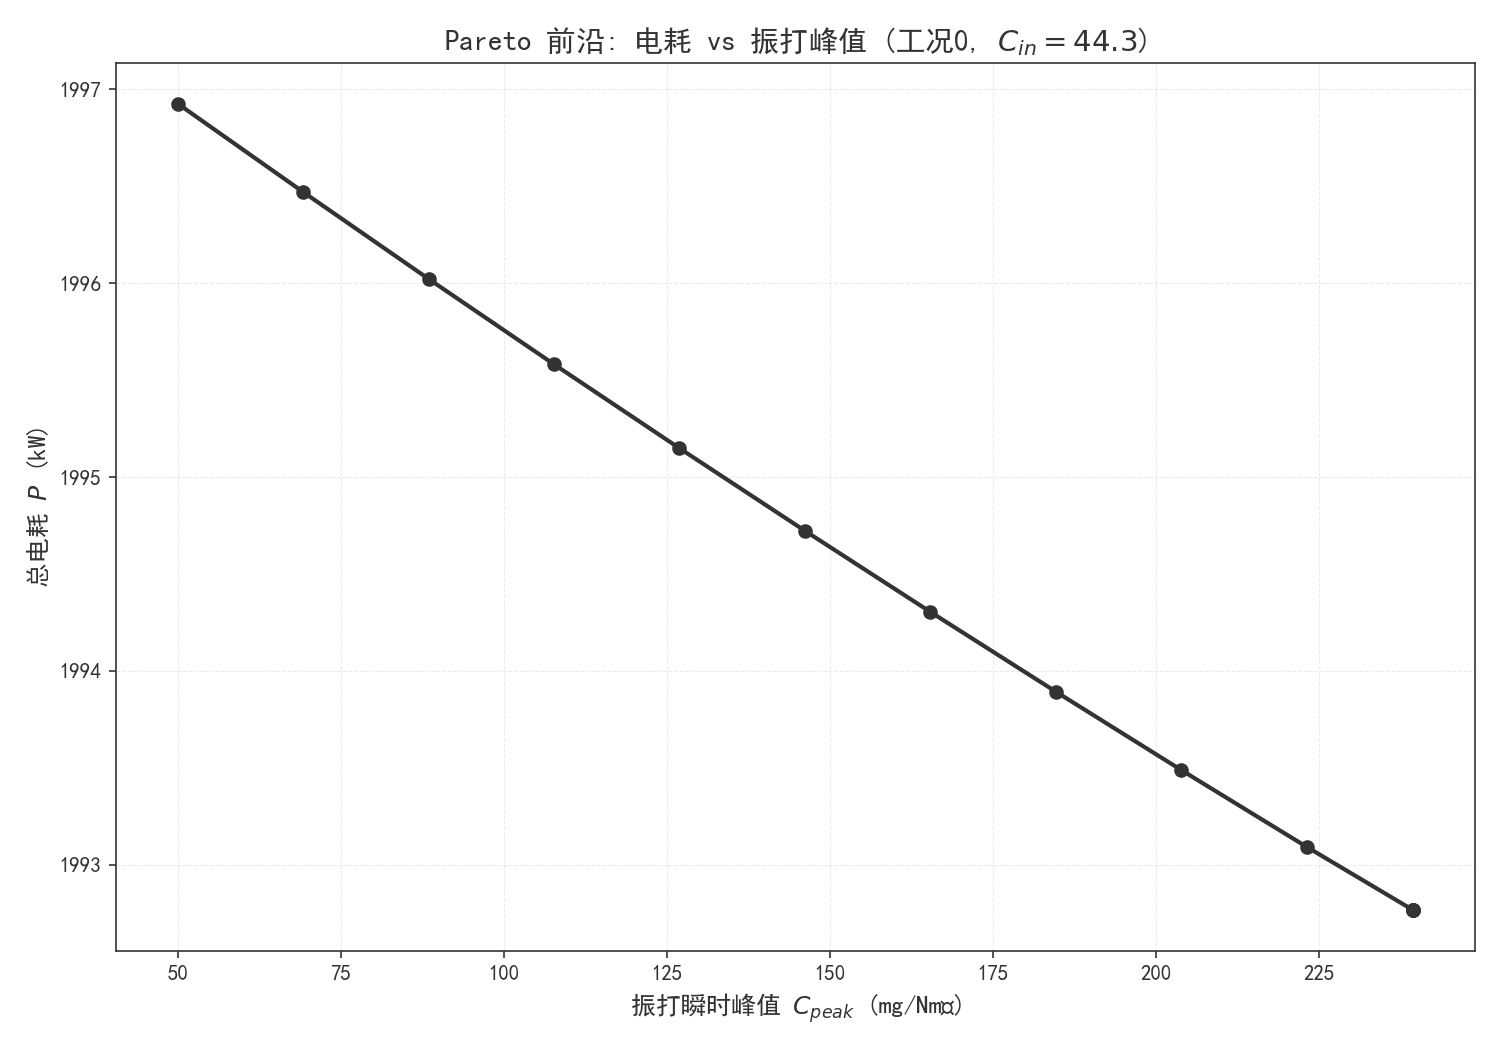
\includegraphics[width=0.85\textwidth]{figures/pareto_front.png}
  \caption{电耗与振打峰值的多目标Pareto前沿}
  \label{fig:pareto_front}
\end{figure}

（2）\textbf{鲁棒优化（机会约束）。}将排放约束改为概率约束$\Pr(C_{out}\leq C_{limit})\geq 1-\varepsilon$，考虑入口条件与模型参数的不确定性，使最优解在扰动下仍以高概率满足排放标准。

（3）\textbf{时序动态优化。}利用7天数据的时序结构，识别日内周期与工况突变点，建立时变工况下的动态优化策略，而非静态分工况寻优。

（4）\textbf{推广至其他除尘设备。}Deutsch方程框架可推广至袋式除尘器（将驱进速度替换为过滤风速）或其他工业ESP（钢铁、火电），仅需重新拟合参数。
